\chapter{Learning to Cluster Documents into Workspaces Using Large Scale Activity Logs}

Google \\

\textbf{Refernce:}~\url{https://dl.acm.org/doi/abs/10.1145/3394486.3403291}~\cite{kong2020learning}

\textbf{Keywords:} user behavior, embeddings, clustering

\section*{Какую задачу решают авторы?}

Авторы решают задачу кластеризации документов в Google Drive в workspace'ы --- отдельные папки, содержащие документы похожие не только по смыслу, но и связанные с конкретными задачами пользователя. \\

У классических подходов к кластеризации документов есть недостатки связанные с тем, что они могут группировать вместе документы одной тематики, но при этом они не учитывают большое количество других факторов.

Например, если пользователь работает над конкретной задачей, то он вполне может использовать документы с разной тематикой. \\

В рамках данной работы, авторы не решают задачу кластеризации напрямую, но обучают document similarity модель, которая для двух документов предсказывает относятся они к одному кластеру или нет.

Используя предсказания модели, авторы используют иерархическую кластеризацию для группировки документов в workspace'ы. \\

\textit{Главный вопрос:} где взять данные для обучение document similarity модели?

На практике, получение датасета достаточного размера, состоящего из пар документов с разметкой от пользователей, может быть довольно сложно. \\

Авторы предлагают способ получить разметку для обучения напрямую из логов активности пользователей --- сводят задачу к weakly supervised варианту.

Основное предположение, которое позволяет получить weak разметку --- если пользователь выполнял действия с документами с небольшой разницей во времени (\textit{co-access}), то скорее всего эти документы относятся к одной задаче, над которой работает пользователь. \\

Авторы в онлайне сравнивают свое решение с классическими unsupervised подходами для кластеризации документов, и показывают, что предлагаемое решение существенно лучше бэйслайнов.

\section*{Как решают?}

Рассмотрим сначала детальнее то как авторы предлагают получать weak разметку, а затем на предлагаемую в статье document similarity модель.

\subsection*{Activity-Based Labels and Weak Supervision}

Для получения разметки, авторы отталкиваются от предположения о похожести документов, с которыми пользователь работал в течении небольшого промежутка времени.

Два документа считаются co-accessed, и получают $label = 1$, если были открыты с разницей во времени не больше двух минут. \\

\begin{wrapfigure}{r}{0.5\textwidth}
    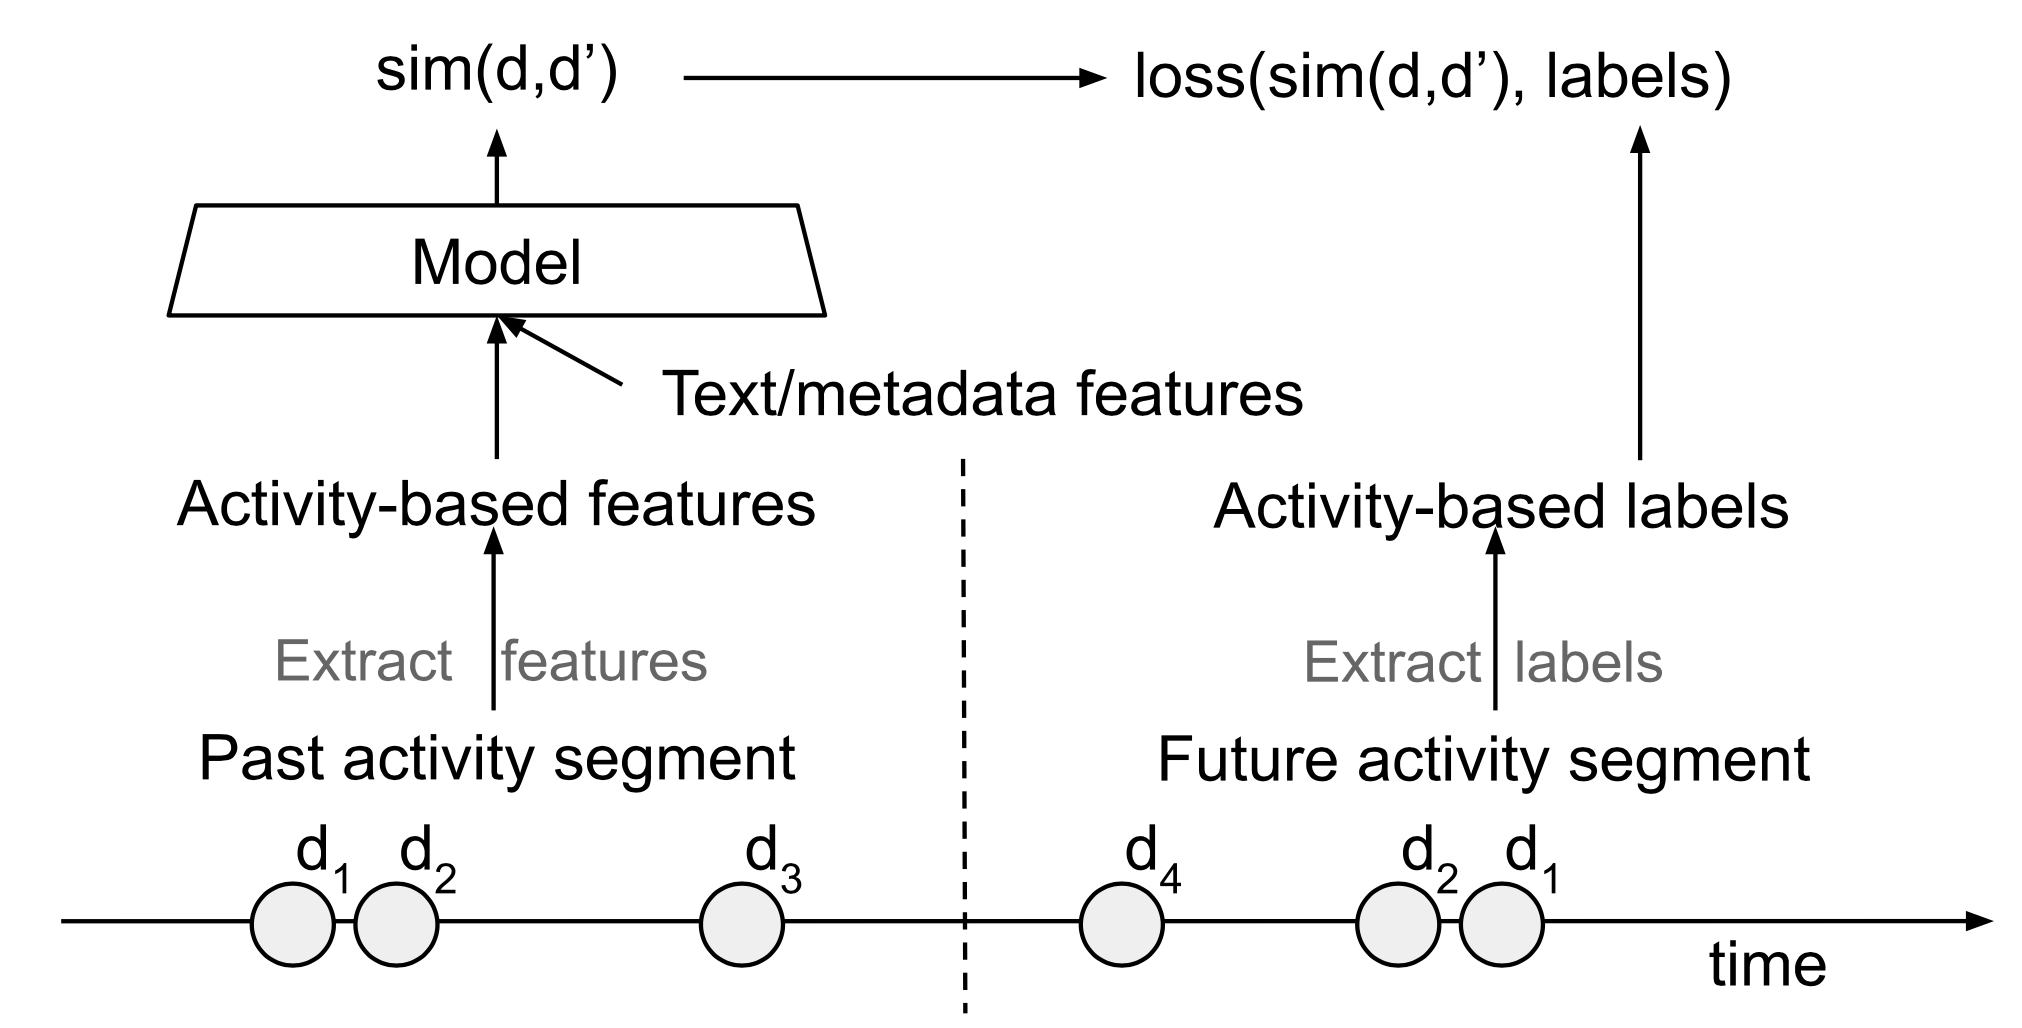
\includegraphics[width=0.99\linewidth]{images/dsm_labels.png}
    \caption{\footnotesize{Past and future activity segments used for extracting activity-based features and labels respectively}}
    \label{fig:dsm_labels}
\end{wrapfigure}
На рисунке~\ref{fig:dsm_labels} показано на каких данных обучается document similarity модель. \\

По сути, вся активность пользователя делиться на две части: первая используется для построения признаков и обучения document similarity модели, а вторая --- для получения разметки. \\

Документы считаются похожими, если они были co-accessed в рамках второй части активности пользователя.

\subsection*{Document Similarity Model}

Рассмотрим подробнее как выглядит модель (см. Рисунок~\ref{fig:dsm}).

\begin{figure}[ht]
    \centering
    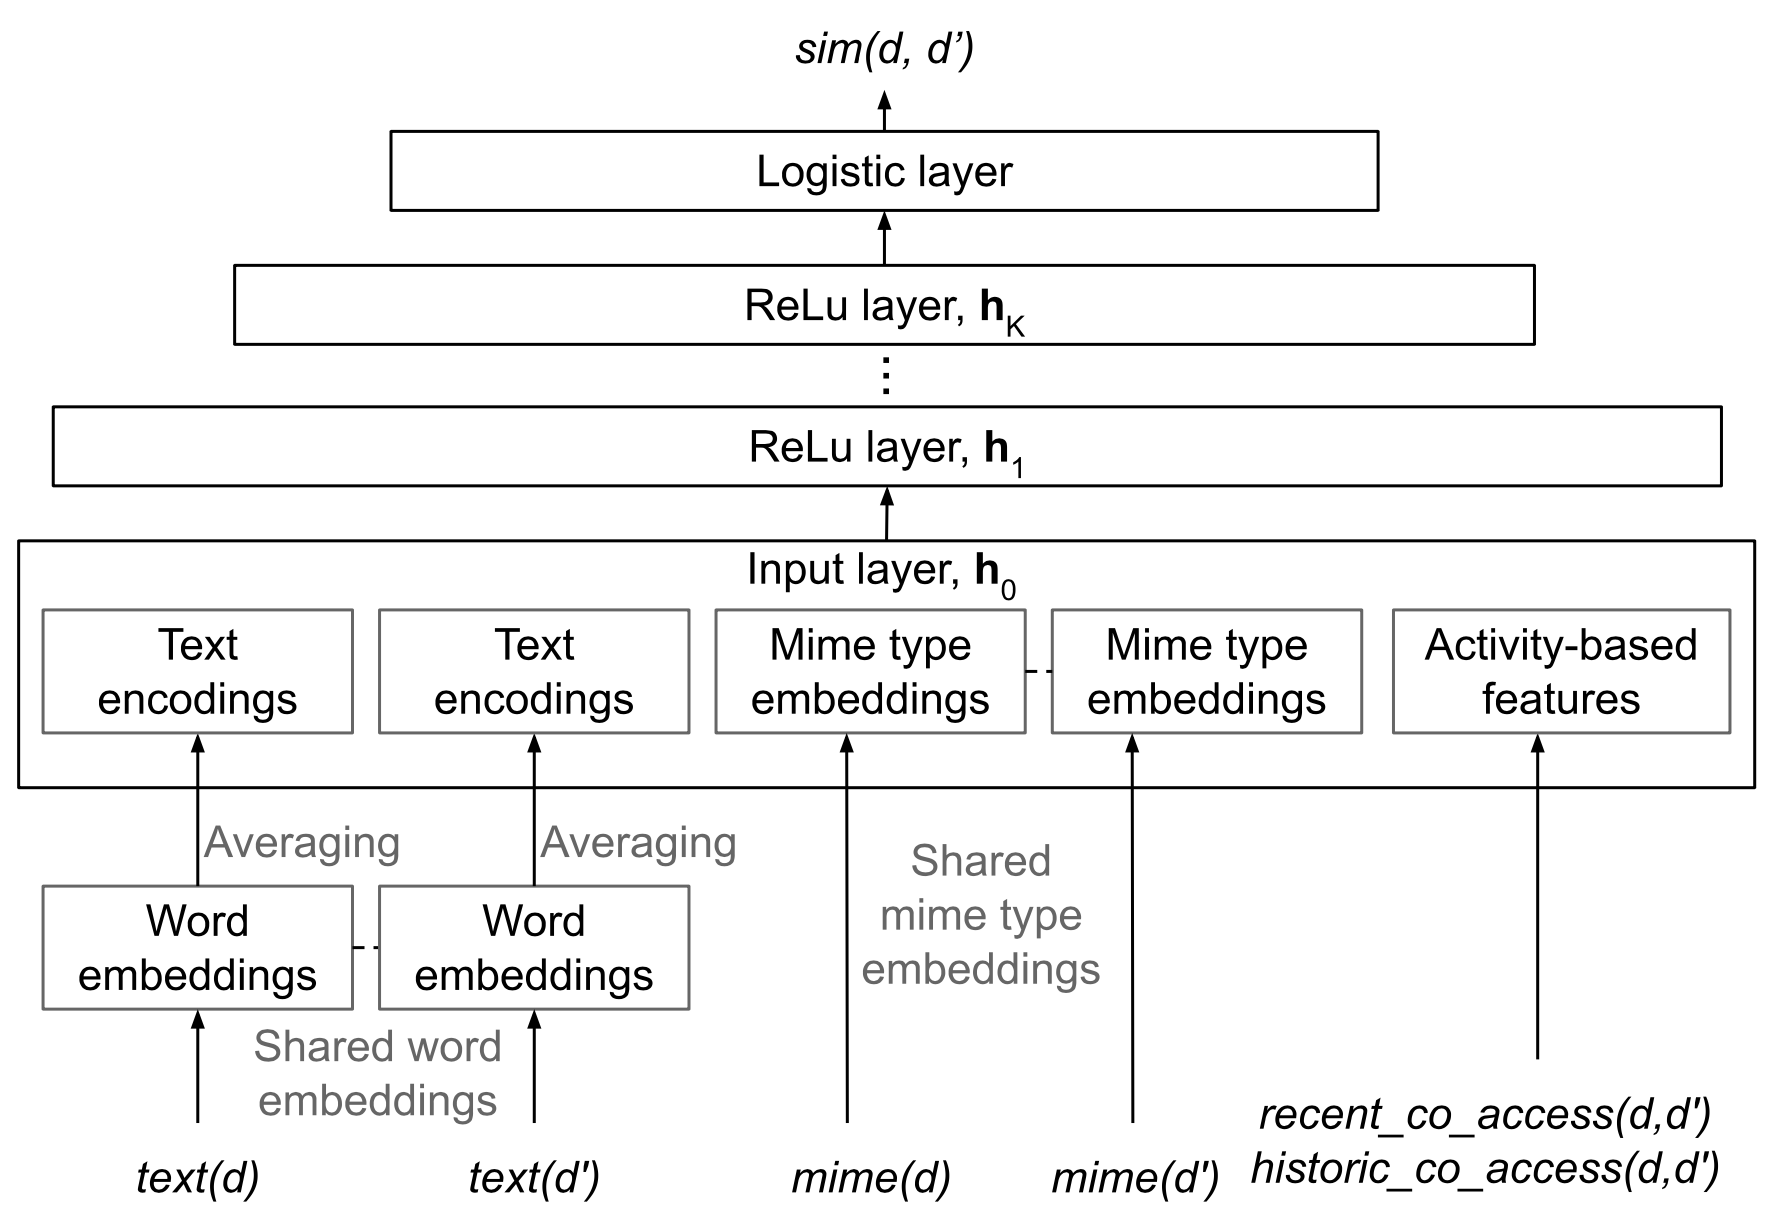
\includegraphics[width=0.7\linewidth]{images/dsm.png}
    \caption{\footnotesize{Document Similarity Model}}
    \label{fig:dsm}
\end{figure}

Список признаков, на которых обучается модель:

\begin{itemize}
    \item \textbf{Text features}
        \begin{itemize}
            \item $text(d)$ - text content for document $d$
            \item $text(d')$ - text content for document $d'$
        \end{itemize}
    \item \textbf{Metadata features}
        \begin{itemize}
            \item $mime(d)$ - MIME type of the document $d$
            \item $mime(d')$ - MIME type of the document $d'$
        \end{itemize}
    \item \textbf{Activity-based features}
        \begin{itemize}
            \item $recent\_co\_accesses(d, d')$ - number of co-accesses between $d, d'$ in the past 2 weeks
            \item $historic\_co\_accesses(d, d')$ - number of co-accesses between $d, d'$ in the past 4 weeks
        \end{itemize}
    \item \textbf{Human and activity-based labels}
        \begin{itemize}
            \item $co\_cluster(d, d')$ - human labels on whether $d, d'$ should be clustered together in a workspace
            \item $future\_co\_accesses(d, d')$ - number of co-accesses between $d, d'$ in the future week
        \end{itemize}
\end{itemize}

Авторы показывают, что дополнительное использование Activity-based  признаков существенно улучшает качество модели, то есть полезно использовать не только признаки связанные с документами, но и информацию о том как пользователь с ними взаимодействовал. \\

DSM обучается минимизируя, привычный для задачи бинарной классификации, Binary Cross-Entropy Loss.

\subsection*{Experiments}

Авторы удтверждают, что documents similarity модель обученная на weak разметке, по качеству не уступает моделе, обученной на разметке от пользователей. \\

Кроме того, авторы проводят онлайн эксперимент и оценивают качество предложенного алгоритма кластеризации со следующими бэйслайнами:

\begin{itemize}
    \item Topicality - для документов обучаются эмбеддинги, которые потом кластеризуются
    \item Calendar - относит в один кластер документы, прикрепленные к одному событию в календаре
    \item Favorites - группирует вместе документы, которые пользователь открывает наиболее часто
\end{itemize}

По результатам экспериментов, предложенный подход работает намного лучше бэйслайнов.

\section*{Мое мнение}

Красивый и простой способ извлечения weak лэйблов, для обучения модели похожести документов, из большого количества логов активности пользователя.